\documentclass{beamer}
%
% Choose how your presentation looks.
%
% For more themes, color themes and font themes, see:
% http://deic.uab.es/~iblanes/beamer_gallery/index_by_theme.html
%
\mode<presentation>
{
  \usetheme{default}      % or try Darmstadt, Madrid, Warsaw, ...
  \usecolortheme{beaver} % or try albatross, beaver, crane, ...
  \usefonttheme{default}  % or try serif, structurebold, ...
  \setbeamertemplate{navigation symbols}{}
  \setbeamertemplate{caption}[numbered]
} 

\usepackage[english]{babel}
\usepackage[utf8x]{inputenc}
\usepackage{hyperref}
\hypersetup{
    colorlinks=true,
    linkcolor=blue,
    filecolor=magenta,      
    urlcolor=blue,
}

\title[Design Considerations]{Design Considerations}
\author{Andrés Pérez}
\institute{Digital Lutherie\\Master en Música para Experiencias del Entretenimiento\\ENTI-UB}
\date{2018/2019}

\newcommand\blfootnote[1]{%
  \begingroup
  \renewcommand\thefootnote{}\footnote{#1}%
  \addtocounter{footnote}{-1}%
  \endgroup
}

\AtBeginSection[]
{
\begin{frame}{Outline}
    \tableofcontents[currentsection] 
\end{frame}
}

\begin{document}

\begin{frame}
  \titlepage
\end{frame}



\begin{frame}{Outline}
 \tableofcontents
\end{frame}

%%%%%%%%%%%%%%%%%%%%%%%%%%%%%%%%%%%%%%%%%%%%%%%%%%
%%%%%%%%%%%%%%%%%%%%%%%%%%%%%%%%%%%%%%%%%%%%%%%%%%
%%%%%%%%%%%%%%%%%%%%%%%%%%%%%%%%%%%%%%%%%%%%%%%%%%
\section{Design Cycle}

\begin{frame}{Design Cycle}
    Waterfall Model
    \begin{figure}[h]
        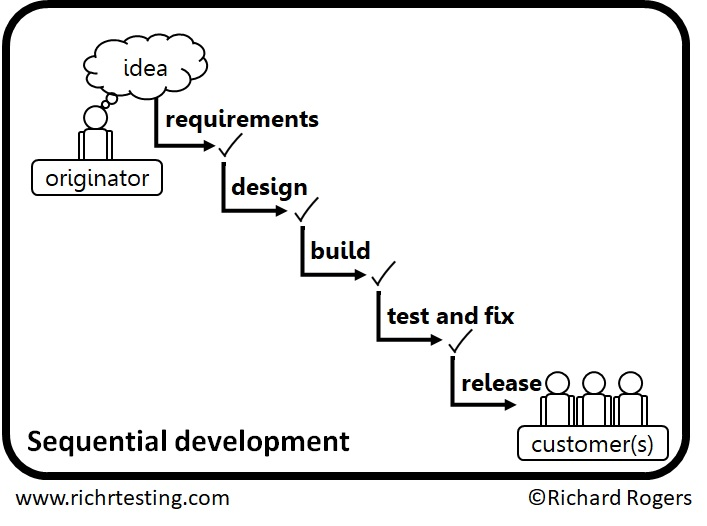
\includegraphics[width=0.75\textwidth]{sequential1.jpg}
    \end{figure}
\end{frame}

\begin{frame}{Design Cycle}
    Iterative Model
    \begin{figure}[h]
        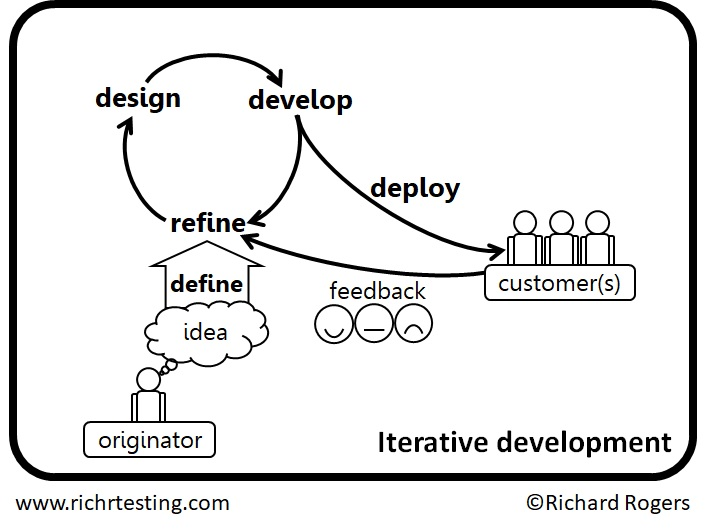
\includegraphics[width=0.75\textwidth]{iterative1.jpg}
    \end{figure}
\end{frame}

\begin{frame}{Design Cycle}
    Questions about the Iterative Model:
    \begin{itemize}
        \item How to evaluate? (again)
        \item Who are the "customers"?
    \end{itemize}
\end{frame}

\begin{frame}{Design Cycle}
    Who are the "customers"?\\
    \vspace{5mm}
    "New standards may not be essential for the creation of new music; perhaps even \textbf{the concept of musical instruments just an old romantic burden} that would be better left aside [...]. New digital instruments conceived holistically and not as a conglomerate of several interchangeable components are scarce; even worse, \textbf{in most cases they are only performed by their creators}."\footnote{Jordà, S. (2007). Interactivity and live computer music. Computer Music Journal.}
\end{frame}

\begin{frame}{Design Cycle}
    Who are the "customers"?\\
    \vspace{5mm}
    \begin{itemize}
        \item Which is/was the last "successful" DMI...?\\
        \item Which is/was the last "successful" non-digital instrument...?
    \end{itemize}
\end{frame}


\section{Output Diversity}

\begin{frame}{Output Diversity}
    Jordà's classification (2007):\footnote{Jordà, S. (2004). Digital Instruments and Players : Part II – Diversity, Freedom and Control, (January 2004).}
    \begin{itemize}
        \item Macro-diversity
        \item Mid-diversity
        \item Micro-diversity
    \end{itemize}
\end{frame}

\begin{frame}{Output Diversity}
    Jordà's classification (2007)\\
    \vspace{5mm}
    Macro-diversity (MacD)
    \begin{itemize}
        \item Context flexibility/versatility
        \item Generic vs specialized 
        \item Correlation with player's expertise level
    \end{itemize}
\end{frame}

\begin{frame}{Output Diversity}
    Jordà's classification (2007)\\
    \vspace{5mm}
    Mid-diversity (MidD)
    \begin{itemize}
        \item Inter-performance diversity
        \item Low MidD: 
        \begin{itemize}
            \item \textit{"Always playing the same piece"}
            \item \textit{"Good for fun but not to be taken too seriously"}
        \end{itemize} 
    \end{itemize}
\end{frame}


\begin{frame}{Output Diversity}
    Jordà's classification (2007)\\
    \vspace{5mm}
    Micro-diversity (MicD)
    \begin{itemize}
        \item Intra-performance diversity
        \item Nuances: potential for virtuosi
        \item Expressivity
    \end{itemize}
\end{frame}



\section{Multithread / Shared Control}

\begin{frame}{Multithread / Shared Control}
    Music temporal scale
    \begin{figure}[h]
        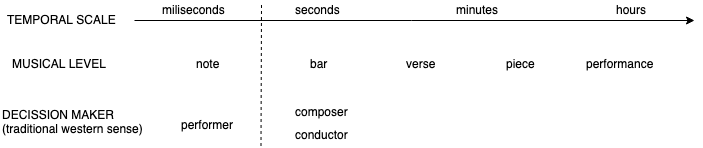
\includegraphics[width=\textwidth]{temporal_scale.png}
    \end{figure}
\end{frame}

\begin{frame}{Multithread / Shared Control}
    \begin{itemize}
        \item Traditional instruments require continuous focus
        \item Traditional instruments affect up to note level (MicD)
    \end{itemize}
    \vspace{5mm}
    But... DMIs do not need to follow these limitations!
\end{frame}

\begin{frame}{Multithread / Shared Control}
    Multithread
    \begin{itemize}
        \item Focusing on several musical aspects at different times
    \end{itemize}
    \vspace{5mm}
    Shared Control
    \begin{itemize}
        \item Leave some decision-making to the computer
    \end{itemize}
    \vspace{5mm}
    Towards a conductor/composer perspective.
\end{frame}



\section{Apprenticeship}

\begin{frame}{Apprenticeship}
    Interaction modes with music performance are broad...
\end{frame}

\begin{frame}{Apprenticeship}
    \begin{figure}[h]
        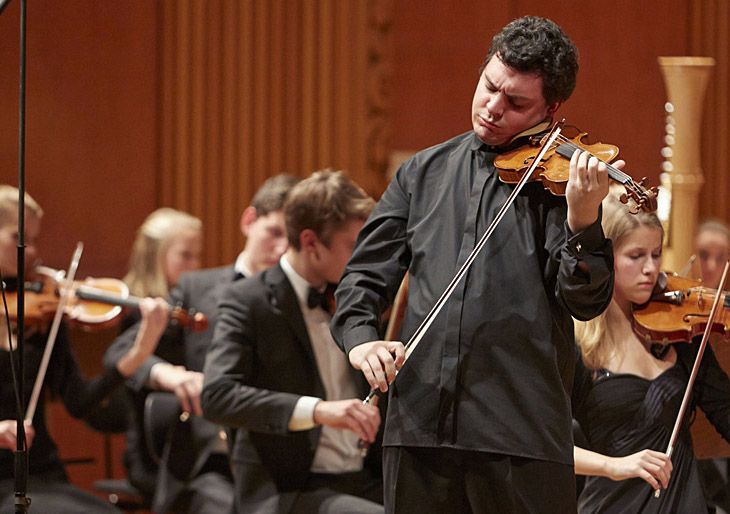
\includegraphics[width=\textwidth]{concertino.jpg}
    \end{figure}
\end{frame}

\begin{frame}{Apprenticeship}
    \begin{figure}[h]
        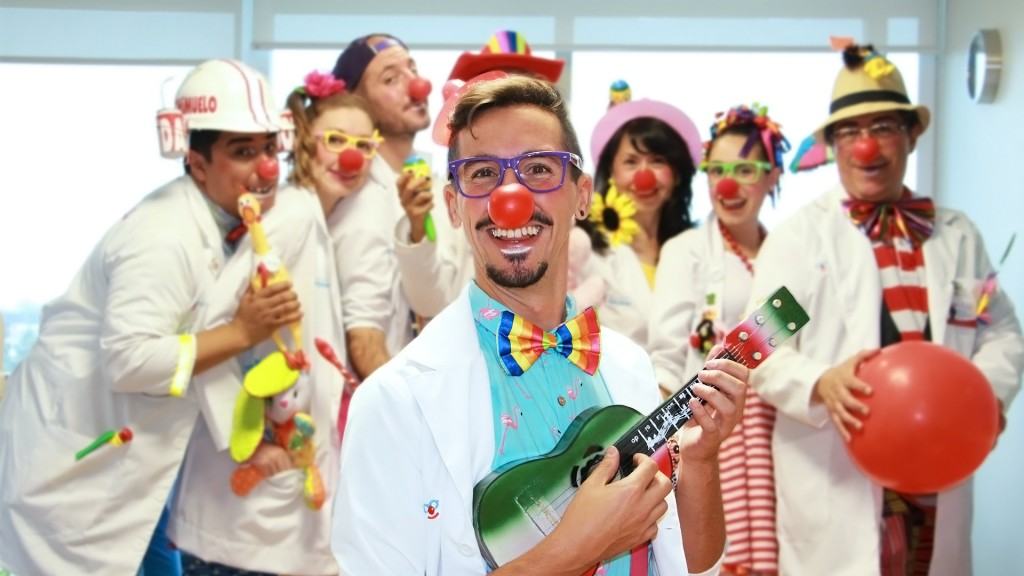
\includegraphics[width=\textwidth]{payasos.jpg}
    \end{figure}
\end{frame}

\begin{frame}{Apprenticeship}
    \begin{figure}[h]
        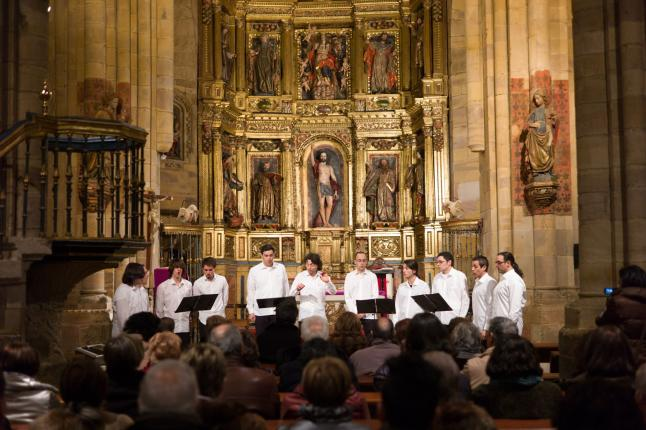
\includegraphics[width=\textwidth]{coro.jpeg}
    \end{figure}
\end{frame}

\begin{frame}{Apprenticeship}
    \begin{figure}[h]
        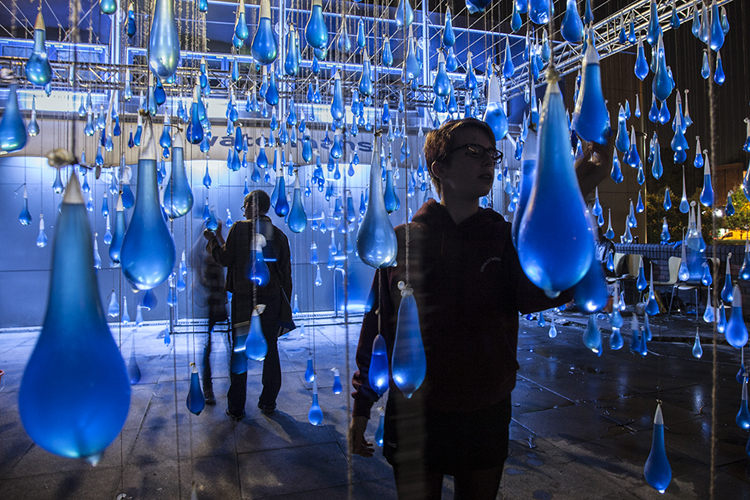
\includegraphics[width=\textwidth]{installation.jpg}
    \end{figure}
\end{frame}

\begin{frame}{Apprenticeship}
    \begin{figure}[h]
        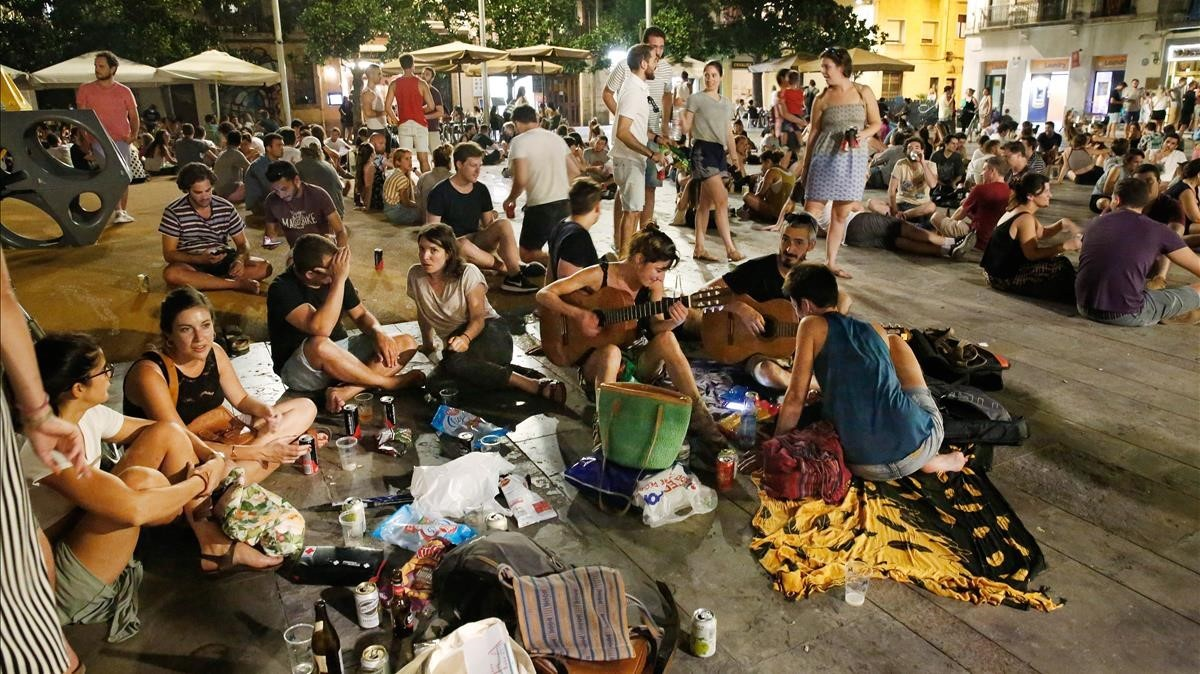
\includegraphics[width=\textwidth]{sol.jpg}
    \end{figure}
\end{frame}

\begin{frame}{Apprenticeship}
    ... so, different people in different moments have different requirements from instruments!
\end{frame}

\subsection{Learning Curve}

\begin{frame}{Apprenticeship - Learning Curve}
    \begin{figure}[h]
        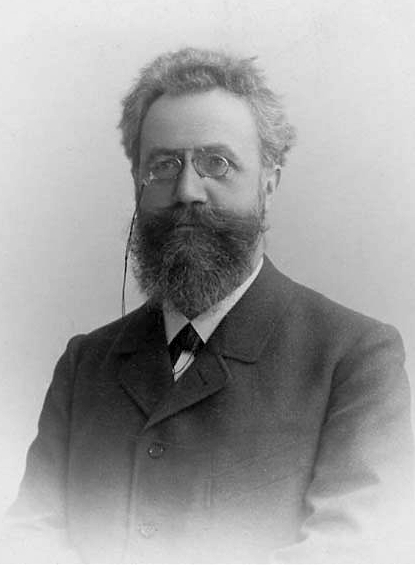
\includegraphics[width=0.5\textwidth]{Ebbinghaus2.jpg}
    \end{figure}
\end{frame}

\begin{frame}{Apprenticeship - Learning Curve}
    Learning Curve (Ebbinghaus, 1885)\\
    \vspace{5mm}
    \textit{"A learning curve is a graphical representation of how an increase in learning (measured on the vertical axis) comes from greater experience (the horizontal axis)."}\footnote{Wikipedia. Learning Curve. Accessed 19/02/2019}
\end{frame}

\begin{frame}{Apprenticeship - Learning Curve}
    \begin{figure}[h]
        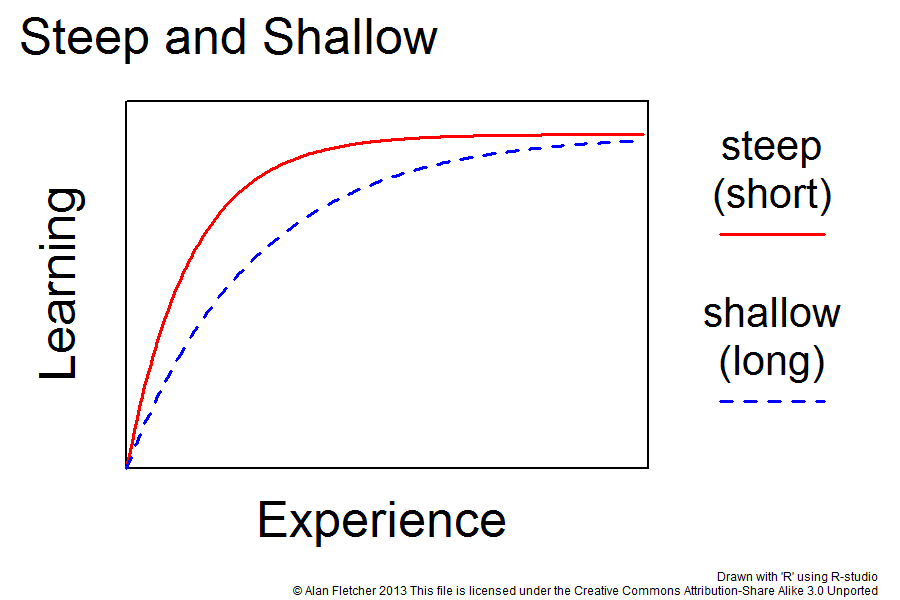
\includegraphics[width=0.8\textwidth]{steepshallow.png}
    \end{figure}\blfootnote{By Alanf777 - Own work, CC BY-SA 3.0, https://commons.wikimedia.org/w/index.php?curid=25252383}
\end{frame}

\begin{frame}{Apprenticeship - Learning Curve}
    \begin{figure}[h]
        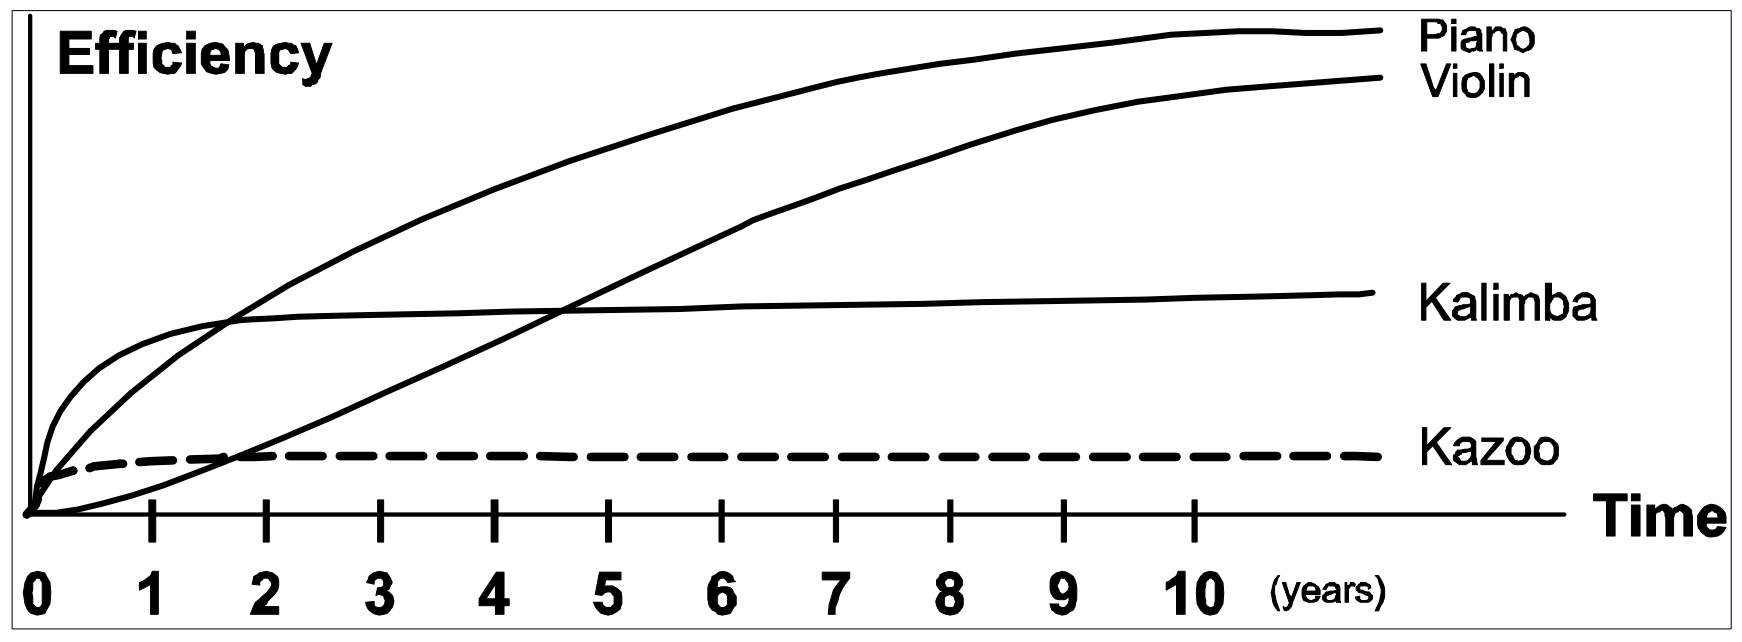
\includegraphics[width=\textwidth]{learningsergi.png}
    \end{figure}\blfootnote{Jordà, S. Digital Instruments and Players : Part I – Efficiency and Apprenticeship (2004).}
\end{frame}

\begin{frame}{Apprenticeship - Learning Curve}
    Some important timestamps:
    \begin{itemize}
        \item \textit{Rewarding Point}\footnote{Levitin D.J. et al. Control parameters for musical instruments: a foundation for new mappings of gesture to sound. Organised Sound (2002)}
        \begin{itemize}
            \item Enough skills to enjoy playing an instrument.
        \end{itemize}
        \item \textit{Mastering Point}
        \begin{itemize}
            \item Time to completely master an instrument.
            \item Usually taken as 10 years for the first acoustic instrument.\footnote{Lehmann, A.C. The Acquisition of Expertise in Music: Efficiency of Deliberate Practice as a Moderating Variable in Accounting for Sub-Expert Performance (1997) .}
        \end{itemize}
    \end{itemize}
\end{frame}

\subsection{Efficiency}

\begin{frame}{Apprenticeship - Efficiency}
   \textit{Efficiency (2b)\footnote{Merriam-Webster. Efficiency. https://www.merriam-webster.com/dictionary/efficiency. Accessed 19/02/2019}: \\
   \vspace{5mm}
   The ratio of the useful energy delivered by a dynamic system to the energy supplied to it.}
   \begin{equation*}
       \text{Efficiency} = \frac{\text{Output}}{\text{Input}}
   \end{equation*}
\end{frame}

\begin{frame}{Apprenticeship - Efficiency}
    Musical Instrument Efficiency\footnote{Jordà, S. Digital Instruments and Players : Part I – Efficiency and Apprenticeship (2004).}:
   \begin{equation*}
       \text{Efficiency} = \frac{\text{MusicalOutputComplexity}}{\text{ControlInputComplexity}}
   \end{equation*}\\
   \vspace{5mm}
   Along time, the control input complexity might also increase..!
\end{frame}

\begin{frame}{Apprenticeship - Efficiency}
    \begin{figure}[h]
        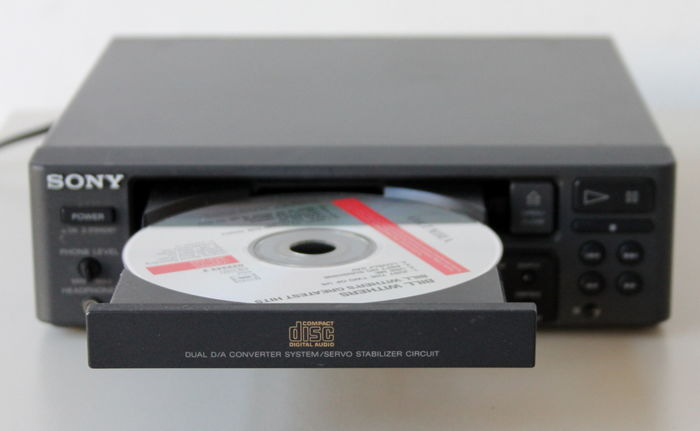
\includegraphics[width=\textwidth]{cd.jpg}
    \end{figure}
\end{frame}

\begin{frame}{Apprenticeship - Efficiency}
    Corrected Musical Instrument Efficiency\footnote{Jordà, S. Digital Instruments and Players : Part I – Efficiency and Apprenticeship (2004).}:\\
    \vspace{5mm}
    \begin{equation*}
       \text{Efficiency} = \frac{\text{MusicalOutputComplexity} \times \text{PerformerFreedom} }{\text{ControlInputComplexity}}
    \end{equation*}\\
\end{frame}

\begin{frame}{Apprenticeship - Efficiency}
    Performer freedom\\
    \vspace{5mm}
    \textit{"A good instrument should not impose its music to its player. A good instrument should not be able to produce only good music! (What is good music anyway?) A good instrument should also be able to produce “terribly bad” music, either at the player’s will or at the player’s misuse."}\footnote{Jordà, S. Digital Instruments and Players : Part I – Efficiency and Apprenticeship (2004).}:
\end{frame}

\begin{frame}{Apprenticeship - Efficiency}
    Playing music vs. Playing with music\\
    \vspace{5mm}
    Musical Instrument vs. Musical Toy
\end{frame}

\begin{frame}{Apprenticeship - Efficiency}
    \begin{figure}[h]
        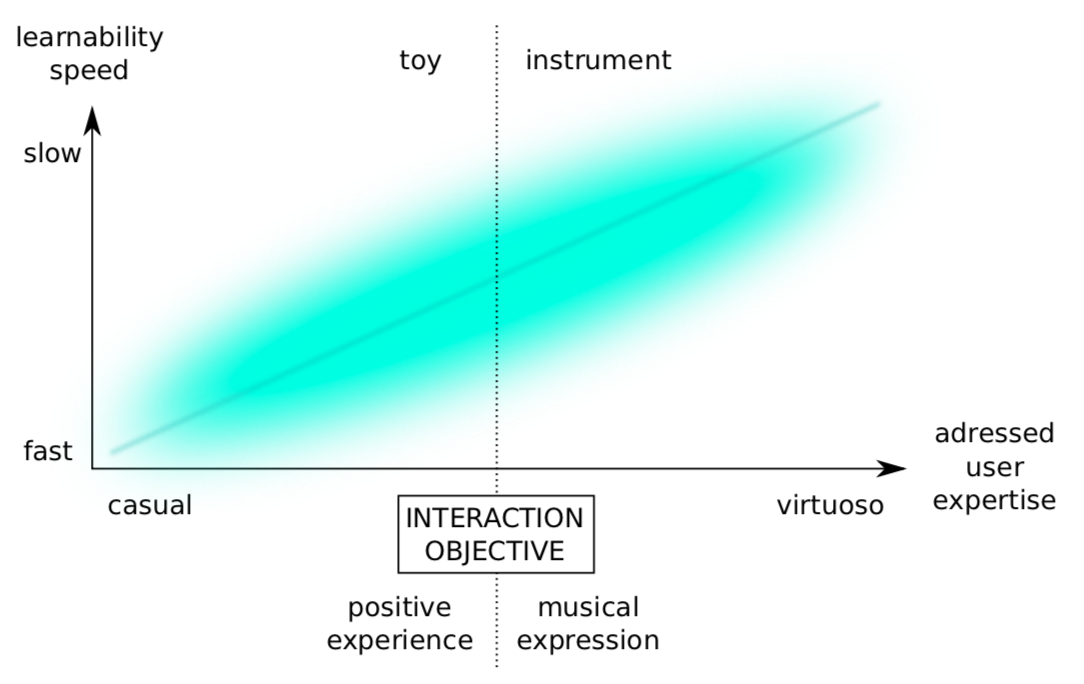
\includegraphics[width=\textwidth]{toy.png}
    \end{figure}
\end{frame}

\end{document}
